\chapter{Экспериментальные исследования}

\section{Цели и задачи экспериментальных исследований}

Формулирование целей и задач экспериментальных исследований.

\section{Методология проведения экспериментов}

Описание методологии проведения экспериментов.

\subsection{Критерии оценки}

Описание критериев оценки эффективности решения.

\subsection{Метрики качества}

Описание используемых метрик качества.

\section{Планирование экспериментов}

Описание плана проведения экспериментов.

\section{Результаты экспериментов}

Представление результатов экспериментальных исследований.

\begin{figure}[H]
\centering
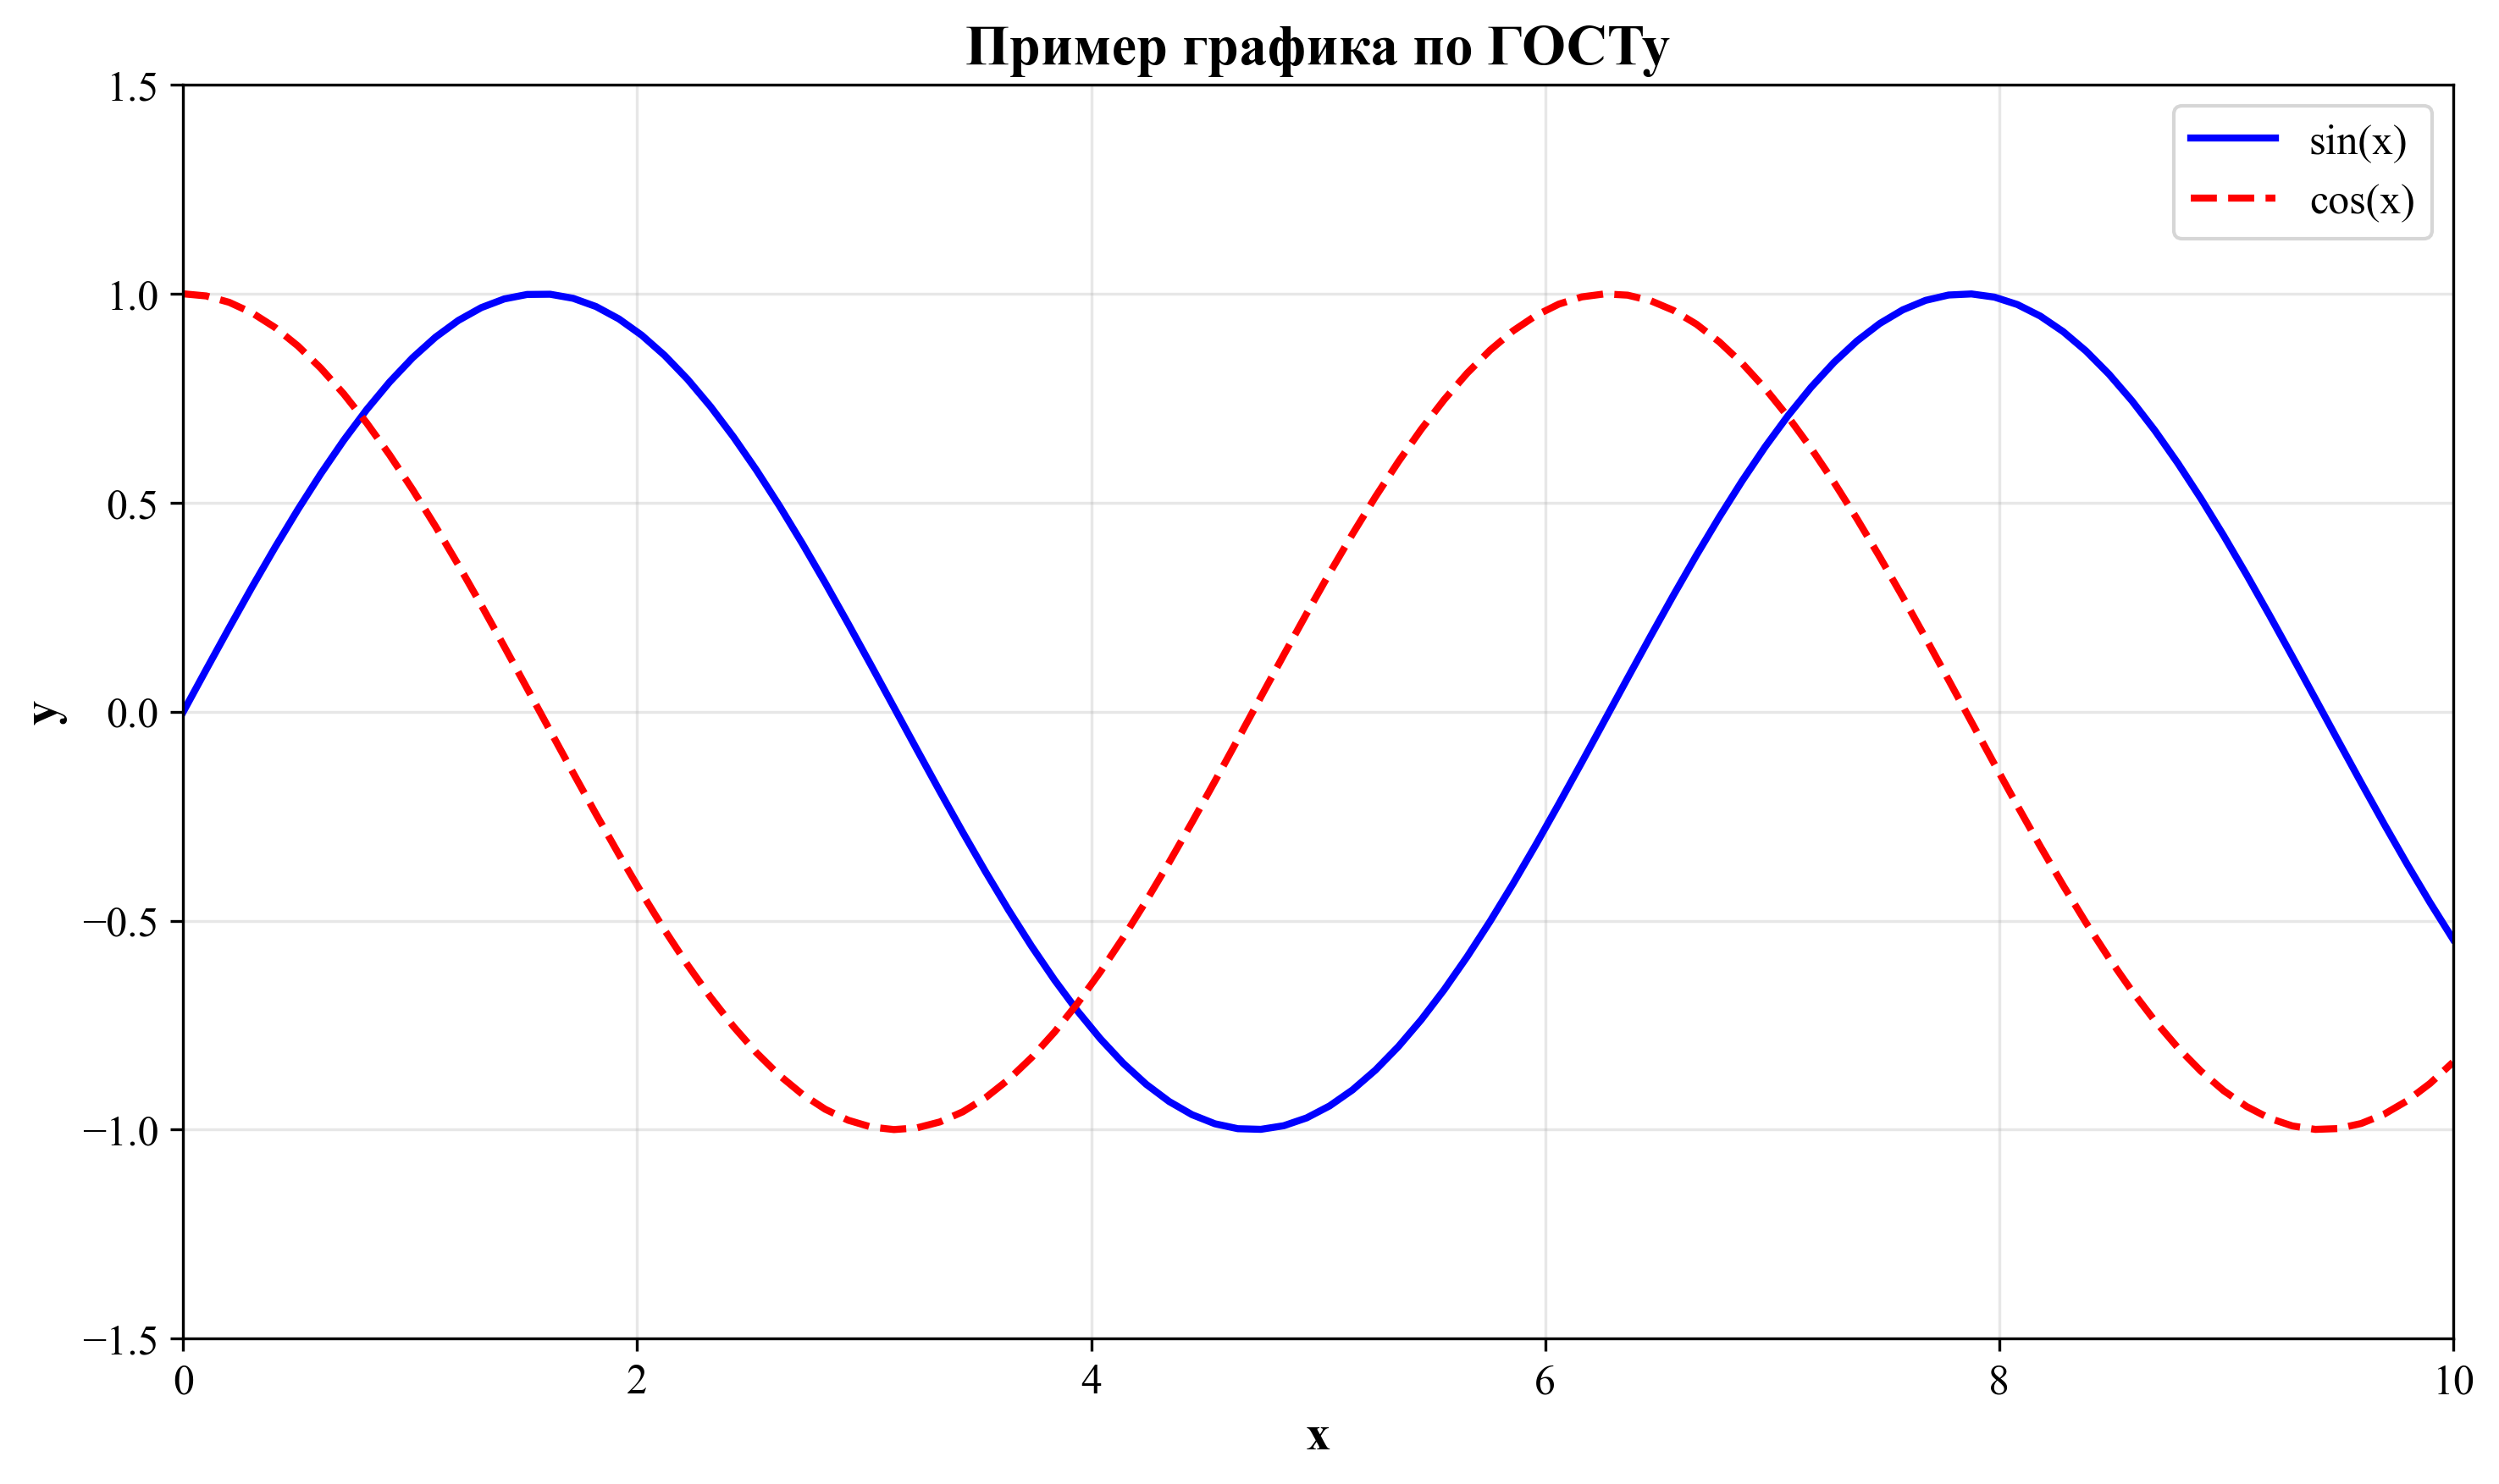
\includegraphics[width=0.8\textwidth]{images/example_plot.png}
\caption{График точности модели в зависимости от количества эпох обучения}
\label{fig:accuracy_plot}
\end{figure}

На рисунке \ref{fig:accuracy_plot} показана динамика изменения точности модели в процессе обучения. Видно, что после 50 эпох модель достигает стабильного уровня точности.

\begin{table}[H]
\centering
\caption{Сравнение различных алгоритмов}
\label{tab:algorithm_comparison}
\begin{tabular}{|l|c|c|c|c|}
\hline
\textbf{Алгоритм} & \textbf{Точность} & \textbf{Время обучения} & \textbf{Время предсказания} & \textbf{Память} \\
\hline
Random Forest & 0.92 & 120 с & 0.1 мс & 50 MB \\
SVM & 0.89 & 300 с & 0.5 мс & 20 MB \\
Neural Network & 0.94 & 600 с & 0.2 мс & 100 MB \\
XGBoost & 0.93 & 180 с & 0.3 мс & 80 MB \\
\hline
\end{tabular}
\end{table}

В таблице \ref{tab:algorithm_comparison} представлено сравнение различных алгоритмов машинного обучения по ключевым метрикам.

\begin{equation}
\text{Accuracy} = \frac{TP + TN}{TP + TN + FP + FN}
\label{eq:accuracy}
\end{equation}

Формула \ref{eq:accuracy} определяет метрику точности классификации, где TP — истинно положительные, TN — истинно отрицательные, FP — ложно положительные, FN — ложно отрицательные результаты.

\begin{CodeBlock}{Python}{Код для вычисления метрик}{lst:metrics_calculation}
from sklearn.metrics import accuracy_score, precision_score, recall_score, f1_score
import numpy as np

def calculate_metrics(y_true, y_pred):
    """Calculate model quality metrics"""
    accuracy = accuracy_score(y_true, y_pred)
    precision = precision_score(y_true, y_pred, average='weighted')
    recall = recall_score(y_true, y_pred, average='weighted')
    f1 = f1_score(y_true, y_pred, average='weighted')
    
    return {
        'accuracy': accuracy,
        'precision': precision,
        'recall': recall,
        'f1_score': f1
    }

# Usage example
y_true = [0, 1, 1, 0, 1]
y_pred = [0, 1, 0, 0, 1]
metrics = calculate_metrics(y_true, y_pred)
print("Accuracy: %.3f" % metrics['accuracy'])
\end{CodeBlock}

В листинге \ref{lst:metrics_calculation} показан код для вычисления основных метрик качества модели машинного обучения.

\subsection{Эксперимент 1}

Описание первого эксперимента и его результатов.

\begin{table}[H]
\centering
\caption{Результаты эксперимента 1}
\begin{tabular}{|l|c|c|c|}
\hline
Параметр & Значение 1 & Значение 2 & Значение 3 \\
\hline
Метрика 1 & 0.95 & 0.87 & 0.92 \\
Метрика 2 & 0.88 & 0.91 & 0.89 \\
\hline
\end{tabular}
\label{tab:exp1}
\end{table}

\subsection{Эксперимент 2}

Описание второго эксперимента и его результатов.

\section{Анализ результатов}

Анализ полученных результатов и их интерпретация.

\subsection{Сравнительный анализ}

Сравнение с существующими решениями.

\subsection{Статистический анализ}

Статистический анализ результатов.

\section{Выводы по главе}

Краткие выводы по экспериментальным исследованиям.
